\directlua{pdf.setminorversion(7)}
\directlua{pdf.inclusioncopyfonts(1)}
\documentclass[a4paper,12pt]{report}
\newcommand{\haupttitel}{Titel der Studienarbeit}
\newcommand{\untertitel}{Untertitel}
\newcommand{\zusammenfassung}{Abstract \/ Subject}
\newcommand{\autorenschaft}{Max Mustermann}
\newcommand{\studiengang}{BSc Information Science}
\newcommand{\matrikelnummer}{00-000-000}
\newcommand{\adresse}{Musterstrasse 1}
\newcommand{\ort}{Musterhausen}
\newcommand{\plz}{0000}
\newcommand{\modul}{WIAGRU}
\newcommand{\email}{max.mustermann@stud.fhgr.ch}
\newcommand{\refe}{Prof. Dr. Eva Mustermann}
\newcommand{\coRefe}{Julian Junke}
\newcommand{\abgabedatum}{TT.MM.YYYY}
\newcommand{\abgabedatumRFC}{YYYY-MM-TT}
\newcommand{\sprache}{de}
\newcommand{\schlagworte}{Keyword 1, Keyword 2}

\usepackage{titlesec, fontspec, polyglossia, setspace, fancyhdr, lscape, caption, subcaption, floatrow, inputenc, graphicx, enumitem, tabularx, colorprofiles, csquotes}

\usepackage[left=3cm,right=2.5cm,top=2.5cm,bottom=2cm]{geometry}
\usepackage[T1]{fontenc}
\usepackage[addtotoc]{abstract}

\usepackage[backend=biber,style=apa,citestyle=apa]{biblatex}
\addbibresource{content/00_assets/quellen.bib}
\let\cite\textcite
\let\citep\parencite

\usepackage[printonlyused]{acronym}

\usepackage{hyphenat}
\hyphenation{Mathe-matik wieder-gewinnen}

\usepackage{chngcntr}
\counterwithout{figure}{chapter}
\counterwithout{table}{chapter}

\graphicspath{{content/00_assets}}

\renewcommand{\thetable}{\arabic{table}}
\renewcommand{\thefigure}{\arabic{figure}}
\renewcommand{\thesubfigure}{\Alph{subfigure}}
\captionsetup[table]{labelfont=it,labelsep=period}
\captionsetup[figure]{labelfont=it,labelsep=period}
% \captionsetup[subfigure]{labelfont=it,labelsep=period,labelformat=simple}
\renewcommand{\arraystretch}{1.3}
\titleformat{\chapter}[block]{\normalfont\large\bfseries}{\thechapter.}{4pt}{}
\titlespacing*{\chapter}{0pt}{0pt}{6pt}
\titleformat{\section}[block]{\normalfont\normalsize\bfseries}{\thesection.}{4pt}{}
\titlespacing*{\section}{0pt}{6pt}{6pt}
\titleformat{\subsection}[block]{\normalfont\normalsize\bfseries}{\thesubsection.}{4pt}{}
\titlespacing*{\subsection}{0pt}{6pt}{6pt}
\setmainfont{Times New Roman}
\setdefaultlanguage[babelshorthands=true,variant=swiss]{german}
% Babelshorthand:
% "` for German-style left double quotes („)
% "' for German-style right double quotes (“)
% "< for French-style left double quotes («)
% "> for French-style right double quotes (»).
% More: https://texdoc.org/serve/polyglossia/0

\setotherlanguages{english,french,italian}
\setstretch{1.3}
\setlength{\parindent}{2.23em}
\fancyhf{}
\renewcommand{\headrulewidth}{0pt}
\pagestyle{fancyplain}
\rfoot{\footnotesize\thepage}

\usepackage[pdfa]{hyperref}
\usepackage{hyperxmp}
\usepackage{embedfile}
\pdfvariable omitcidset=1

%\embedfile[afrelationship={/Source},ucfilespec={main.tex},mimetype={application/x-tex}]{main.tex}

\hypersetup{%
    pdflang=\sprache,
    pdftitle={\haupttitel},
    pdfsubtitle={\untertitel},
    pdfauthor={\autorenschaft},
    pdfdate={\datumBisRFC},
    pdfsubject={\zusammenfassung},
    pdfkeywords={\modul, \schlagworte},
    pdfcontactaddress={\adresse},
    pdfcontactcity={\ort},
    pdfcontactpostcode={\plz},
    pdfcontactphone={\telefon},
    pdfcontactemail={\email},
    colorlinks,
    unicode,
    allcolors=black,
    pdfapart=2,
    pdfaconformance=U
}

%Create an OutputIntent in order to correctly specify colours
\immediate\pdfobj stream attr{/N 3} file{sRGB.icc}
\pdfcatalog{%
  /OutputIntents [
    <<
      /Type /OutputIntent
      /S /GTS_PDFA1
      /DestOutputProfile \the\pdflastobj\space 0 R
      /OutputConditionIdentifier (sRGB)
      /Info (sRGB)
    >>
  ]
}

\begin{document}
\renewcommand{\figurename}{Abb.}
\renewcommand{\tablename}{Tab.}
\renewcommand*\listfigurename{\normalfont\large\bfseries{Abbildungsverzeichnis}}
\renewcommand*\listtablename{\normalfont\large\bfseries{Tabellenverzeichnis}}
\renewcommand*\contentsname{\normalfont\large\bfseries{Inhaltsverzeichnis}}
% Start Vorspann
\pagenumbering{Roman} % Römische Seitenzahl
\begin{titlepage}
    
    \begin{center}
        \huge{Titel der Arbeit der etwas länger ist damit er umbricht. Und eventuell sich sogar auf drei ganze Zeilen verteilt.}\\
         \vfill
        \large{Untertitel Untertitel Untertitel Untertitel Untertitel Untertitel Untertitel Untertitel Untertitel}
    \end{center}
    
    \vfill
    
    \begin{tabbing}
    Verfasser:  \=\hspace*{2.5cm} Max Mustermann\\
                \>\hspace*{2.5cm} Musterstrasse 1\\
                \>\hspace*{2.5cm} 1000 Musterstadt\\
                \>\hspace*{2.5cm} Tel.: 012 345 67 89\\
                \>\hspace*{2.5cm} E-Mail: max.mustermann@stud.fhgr.ch\\
                \\
    Referent:   \>\hspace*{2.5cm} Prof, Dr. Eva Mustermann\\
    Modul:      \>\hspace*{2.5cm} WIAGRU\\
                \\
    Bearbeitungszeitraum: \>\hspace*{2.5cm} tt. Monat Jahr bis tt. Monat Jahr
    \end{tabbing}
    
    \vfill
    
    \begin{center} 
        \textbf{Bern, Monat Jahr}
    \end{center}

\end{titlepage}
\renewcommand{\abstractname}{Abstract}
\begin{abstract}
\thispagestyle{plain}
Abstract
\blindtext
\end{abstract}
\chapter*{Vorwort}
Sit amet mattis vulputate enim nulla aliquet. Risus at ultrices mi tempus imperdiet nulla malesuada pellentesque. Turpis nunc eget lorem dolor sed viverra ipsum nunc aliquet. Turpis egestas integer eget aliquet nibh praesent. Sed euismod nisi porta lorem mollis aliquam ut porttitor leo. Sem viverra aliquet eget sit. Id leo in vitae turpis massa sed elementum tempus egestas. Pharetra vel turpis nunc eget lorem dolor sed viverra ipsum. Velit ut tortor pretium viverra suspendisse potenti nullam ac. Eget sit amet tellus cras adipiscing enim eu turpis. Pulvinar neque laoreet suspendisse interdum consectetur libero. Consequat interdum varius sit amet mattis vulputate enim nulla aliquet. Amet purus gravida quis blandit turpis cursus in hac habitasse. In aliquam sem fringilla ut morbi tincidunt augue. Tellus molestie nunc non blandit massa enim nec. Mi eget mauris pharetra et ultrices neque.

Sit amet mattis vulputate enim nulla aliquet. Risus at ultrices mi tempus imperdiet nulla malesuada pellentesque. Turpis nunc eget lorem dolor sed viverra ipsum nunc aliquet. Turpis egestas integer eget aliquet nibh praesent. Sed euismod nisi porta lorem mollis aliquam ut porttitor leo. Sem viverra aliquet eget sit. Id leo in vitae turpis massa sed elementum tempus egestas. Pharetra vel turpis nunc eget lorem dolor sed viverra ipsum. Velit ut tortor pretium viverra suspendisse potenti nullam ac. Eget sit amet tellus cras adipiscing enim eu turpis. Pulvinar neque laoreet suspendisse interdum consectetur libero. Consequat interdum varius sit amet mattis vulputate enim nulla aliquet. Amet purus gravida quis blandit turpis cursus in hac habitasse. In aliquam sem fringilla ut morbi tincidunt augue. Tellus molestie nunc non blandit massa enim nec. Mi eget mauris pharetra et ultrices neque.
\setcounter{page}{2}
\tableofcontents % Inhaltsverzeichnis
\begingroup
	\renewcommand*{\addvspace}[1]{}
    \newpage
	\listoffigures
	\newpage
	\listoftables
\endgroup
\FakeChapter{Abkürzungsverzeichnis}

\begin{acronym}[LONGESTWORD]\itemsep0pt
    \acro{etc}[Etc.]{Etcetera}
    \acro{zb}[z.B.]{zum Beispiel}
\end{acronym}
% Ende Vorpsann
% Start Textteil
\pagenumbering{arabic} % Arabische Seitenzahl
\chapter{Einleitung}
Sit amet mattis "<vulputate"> enim nulla aliquet. Risus at ultrices mi tempus imperdiet nulla malesuada pellentesque. Turpis nunc eget lorem dolor sed viverra ipsum nunc aliquet. Turpis egestas integer eget aliquet nibh praesent. Sed euismod nisi porta lorem mollis aliquam ut porttitor leo. Sem viverra aliquet eget sit. Id leo in vitae turpis massa sed elementum tempus egestas. Pharetra vel turpis nunc eget lorem dolor sed viverra ipsum. Velit ut tortor pretium viverra suspendisse potenti nullam ac. Eget sit amet tellus cras adipiscing enim eu turpis. Pulvinar neque laoreet suspendisse interdum consectetur libero. Consequat interdum varius sit amet mattis vulputate enim nulla aliquet. Amet purus gravida quis blandit turpis cursus in hac habitasse. In aliquam sem fringilla ut morbi tincidunt augue. Tellus molestie nunc non blandit massa enim nec. Mi eget mauris pharetra et ultrices neque.
\chapter{Erstes Kapitel}
Dies ist eine Vorlage für wissenschaftliche Arbeiten an der FHGR nach \cite{selina_leitfaden_nodate}. \acs{zb} (\acl{zb}) ist eine Abkürzung. Die folgende Abbildung zeigt eine Alpendohle (\ref{fig:alpendohle}).

\begin{figure}[h]
    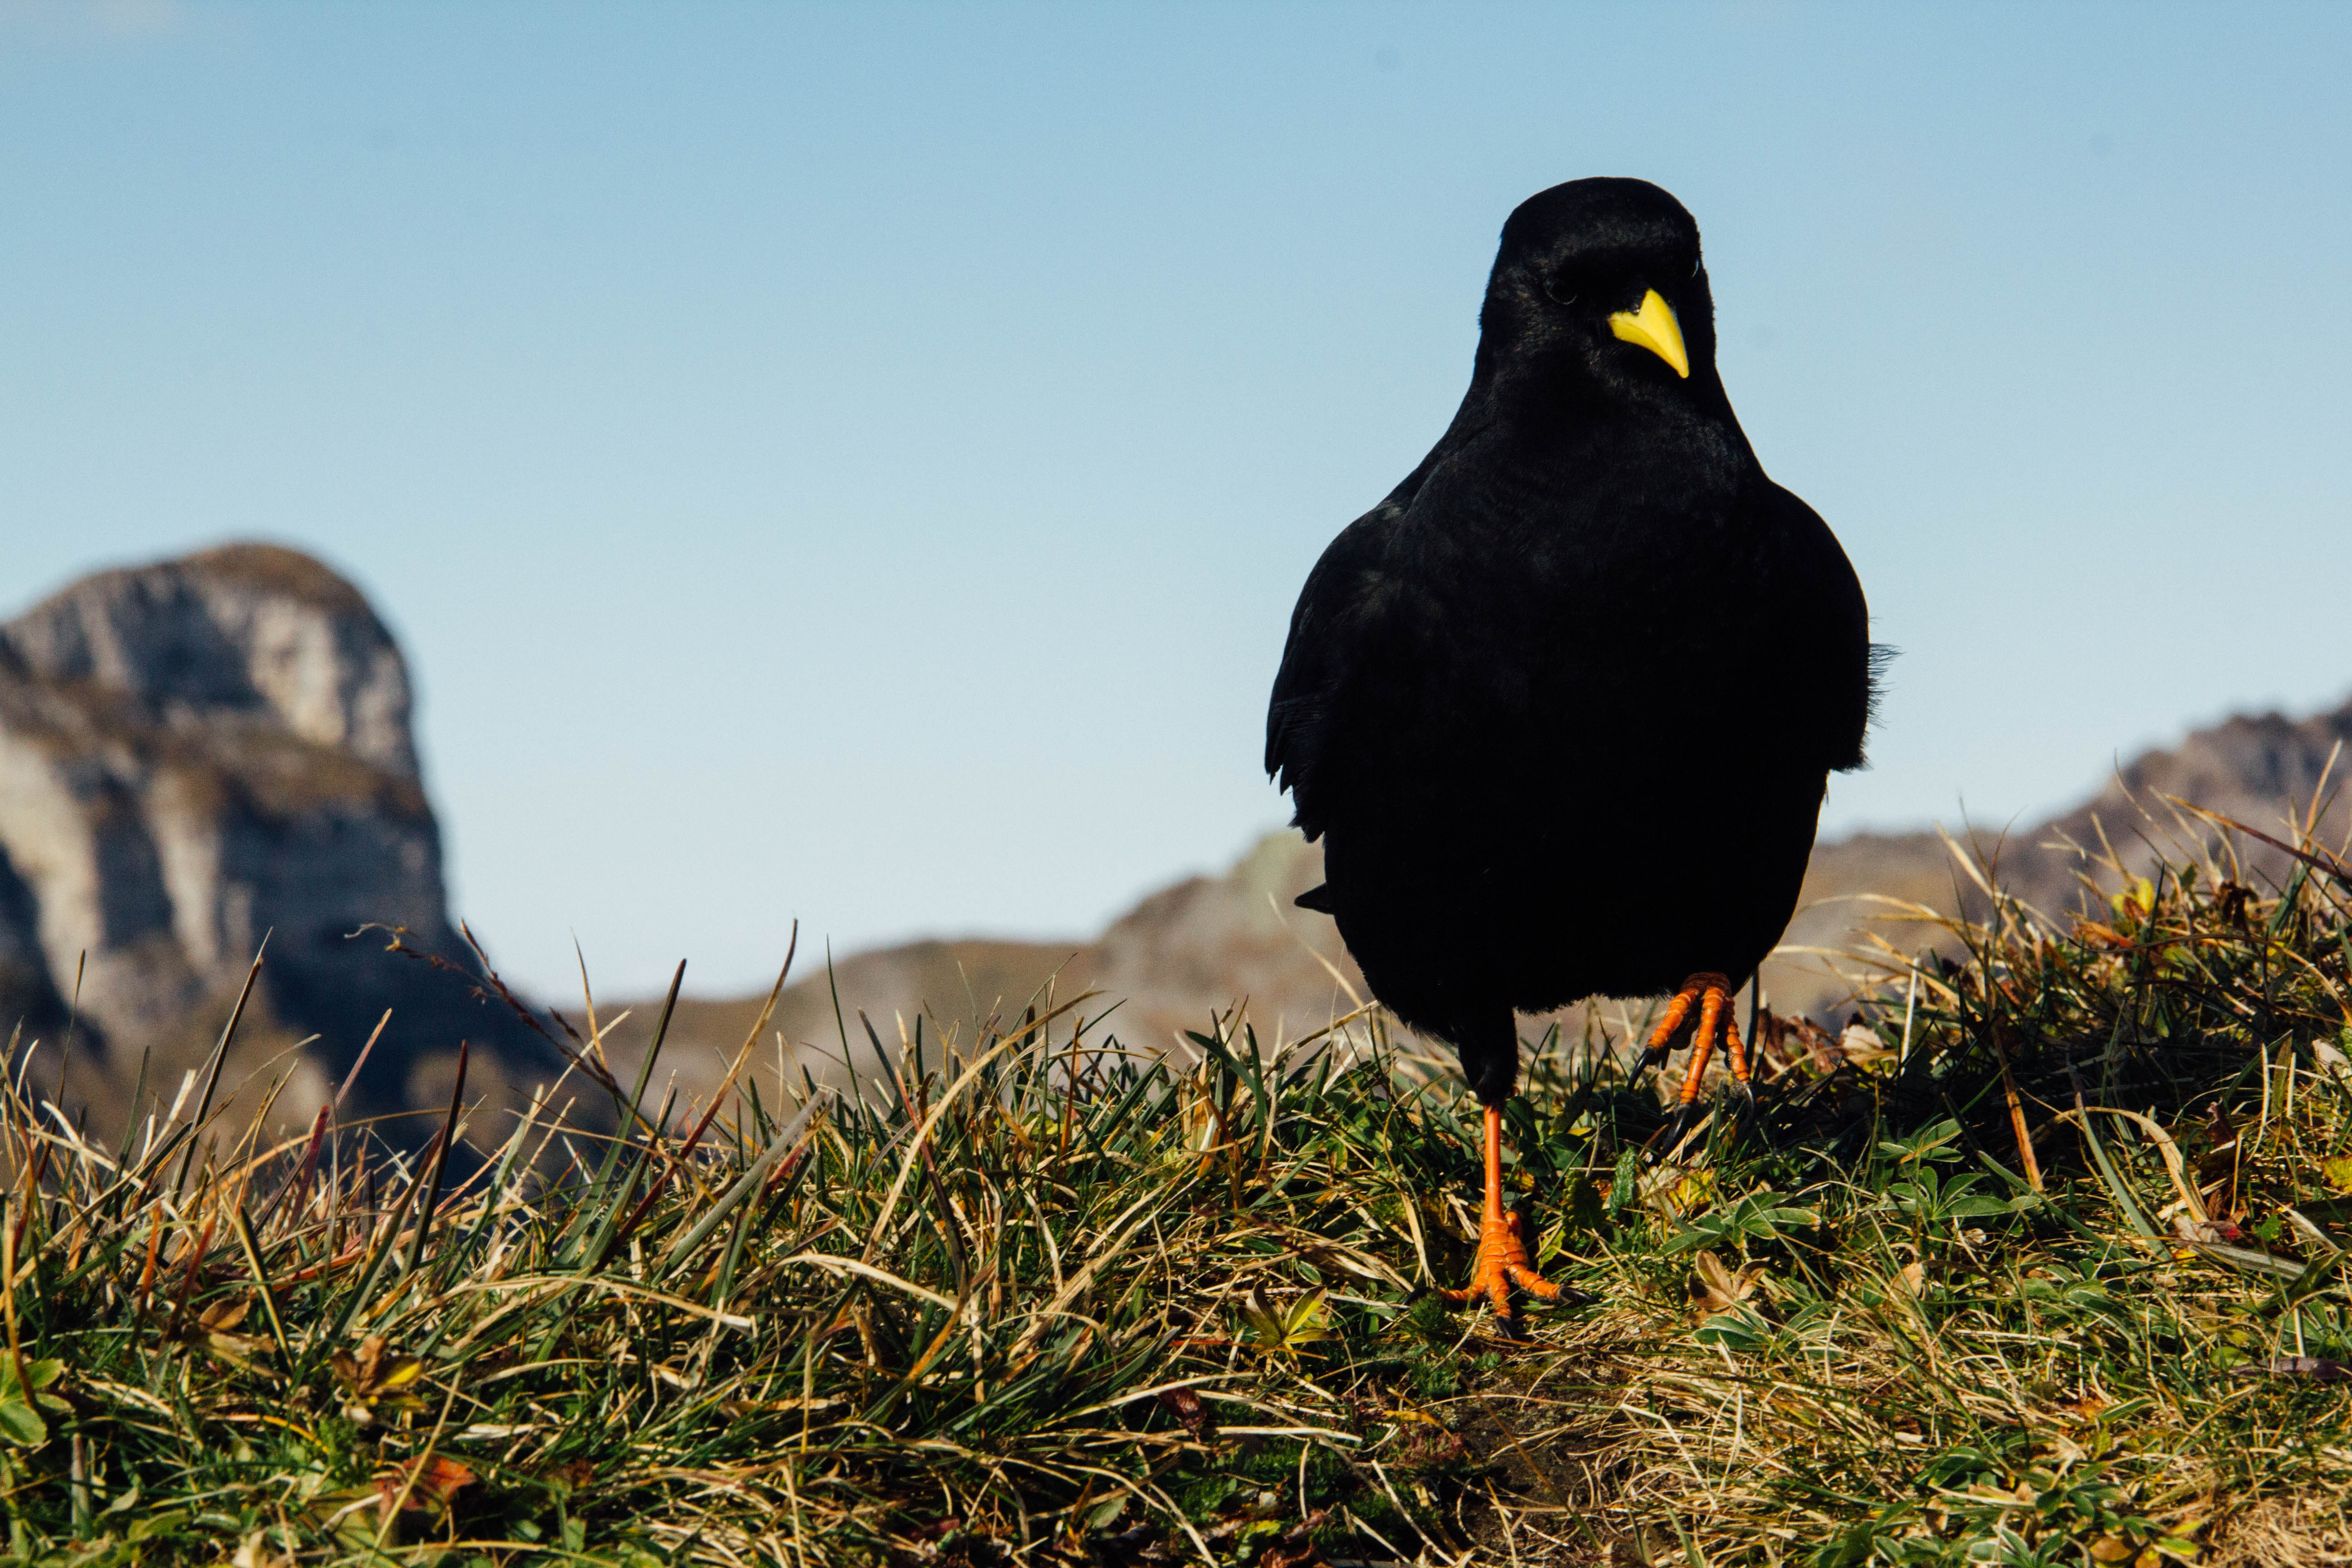
\includegraphics[width=\textwidth]{content/00_assets/alpendohle.jpg}
    \caption{Eine Alpendohle}
    \label{fig:alpendohle}
\end{figure}

\blindtext

\begin{table}[ht]
\begin{tabularx}{\textwidth} {
    >{\raggedright\arraybackslash}X 
    >{\raggedleft\arraybackslash}X 
    >{\raggedleft\arraybackslash}X}
        \hline
        \multicolumn{3}{c}{\textbf{Tabelle}}\\
        \hline
        \textbf{Linksbündig} & \textbf{Rechtsbündig} & \textbf{Rechtsbündig}\\
        \hline
        Lorem & N/A & N/A\\
        Ipsum & 1 499 & 8 512\\
        Dolor & 297 & N/A\\
        Sit & 1 053 & N/A\\
        \hline
        \textbf{Total} & 2 849 & 8 512\\
        \hline
\end{tabularx}
\caption{Beispiel einer Tabelle}.
    \label{tab:tabelle}
\end{table}

\section{Subkapitel}
\blindtext

\section{Subkapitel}
\blindtext
\begin{quote}
    \blindtext
\end{quote}
\blindtext
% Ende Textteil
% Start Nachspann
\printbibliography[heading=bibintoc,title={Literaturverzeichnis}]
\appendix
\FakeChapter{Anhang}{toc}
Sit amet mattis vulputate enim nulla aliquet. Risus at ultrices mi tempus imperdiet nulla malesuada pellentesque. Turpis nunc eget lorem dolor sed viverra ipsum nunc aliquet. Turpis egestas integer eget aliquet nibh praesent. Sed euismod nisi porta lorem mollis aliquam ut porttitor leo. Sem viverra aliquet eget sit. Id leo in vitae turpis massa sed elementum tempus egestas. Pharetra vel turpis nunc eget lorem dolor sed viverra ipsum. Velit ut tortor pretium viverra suspendisse potenti nullam ac. Eget sit amet tellus cras adipiscing enim eu turpis. Pulvinar neque laoreet suspendisse interdum consectetur libero. Consequat interdum varius sit amet mattis vulputate enim nulla aliquet. Amet purus gravida quis blandit turpis cursus in hac habitasse. In aliquam sem fringilla ut morbi tincidunt augue. Tellus molestie nunc non blandit massa enim nec. Mi eget mauris pharetra et ultrices neque.
\thispagestyle{empty}
\noindent
Ich erkläre hiermit, dass ich diese Arbeit selbstständig verfasst und keine anderen als die angegebenen Quellen und erlaubten Hilfsmittel benutzt habe, einschliesslich der Verwendung von KI-Systemen. Alle Stellen, die wörtlich oder sinngemäss aus Quellen entnommen worden sind, habe ich als solche gekennzeichnet. Ich bin den Vorgaben des Leitfadens wissenschaftliches Arbeiten gefolgt. Mir ist bekannt, dass andernfalls die Hochschulleitung zum Entzug der aufgrund meiner Arbeit verliehenen Qualifikation oder des für meine Arbeit verliehenen Titels berechtigt ist\\
\\
\\
\\
Bern, 13.06.2003 \hfill 
\includegraphics[width=2cm]{content/00_assets/unterschrift.png}\\
Ort, Datum \hfill Unterschrift \autorenschaft
% Ende Nachspann
\end{document}

